\documentclass[nobib]{tufte-handout}

\title{Lecture 3: Common graph families, trees, and Cayley's theorem $\cdot$ 1MA020}

\author[Vilhelm Agdur]{Vilhelm Agdur\thanks{\href{mailto:vilhelm.agdur@math.uu.se}{\nolinkurl{vilhelm.agdur@math.uu.se}}}}

\date{24 October 2023}


%\geometry{showframe} % display margins for debugging page layout

\usepackage{graphicx} % allow embedded images
  \setkeys{Gin}{width=\linewidth,totalheight=\textheight,keepaspectratio}
  \graphicspath{{graphics/}} % set of paths to search for images
\usepackage{amsmath}  % extended mathematics
\usepackage{booktabs} % book-quality tables
\usepackage{units}    % non-stacked fractions and better unit spacing
\usepackage{multicol} % multiple column layout facilities
\usepackage{lipsum}   % filler text
\usepackage{fancyvrb} % extended verbatim environments
  \fvset{fontsize=\normalsize}% default font size for fancy-verbatim environments

\usepackage{color,soul} % Highlights for text

% Standardize command font styles and environments
\newcommand{\doccmd}[1]{\texttt{\textbackslash#1}}% command name -- adds backslash automatically
\newcommand{\docopt}[1]{\ensuremath{\langle}\textrm{\textit{#1}}\ensuremath{\rangle}}% optional command argument
\newcommand{\docarg}[1]{\textrm{\textit{#1}}}% (required) command argument
\newcommand{\docenv}[1]{\textsf{#1}}% environment name
\newcommand{\docpkg}[1]{\texttt{#1}}% package name
\newcommand{\doccls}[1]{\texttt{#1}}% document class name
\newcommand{\docclsopt}[1]{\texttt{#1}}% document class option name
\newenvironment{docspec}{\begin{quote}\noindent}{\end{quote}}% command specification environment

\include{mathcommands.extratex}

\begin{document}

\maketitle% this prints the handout title, author, and date

\begin{abstract}
\noindent
We start by introducing a few named families of graphs. Then we introduce the class of \emph{trees}, and prove some results about them. The main result is Cayley's theorem, which counts the number of labelled trees on $n$ vertices.
\end{abstract}

\section{Common graph families}

We warm up today by giving names to some common families of simple graphs that we will see reappearing throughout the course. They are illustrated in Figure \ref{fig:graph_families}.

\begin{figure}
  \centering
  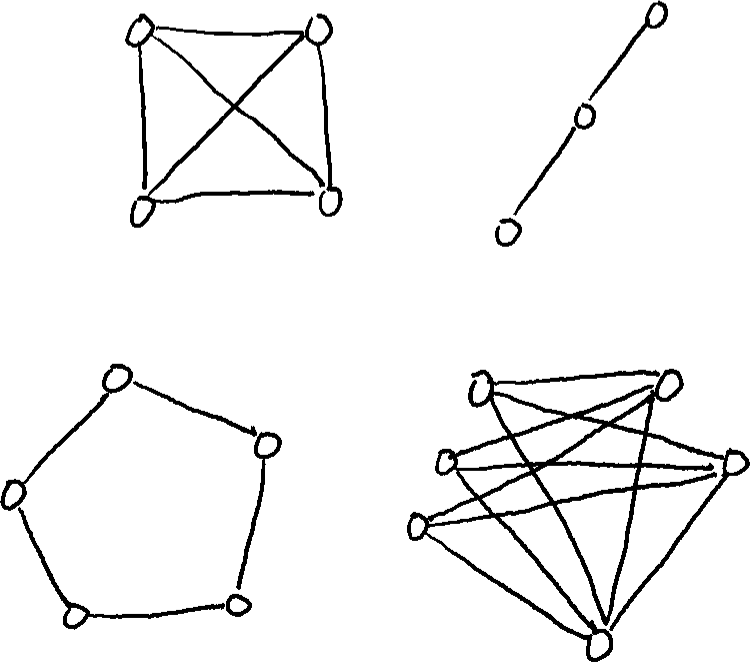
\includegraphics[width=0.5\textwidth]{graphics/L3_trees/graph_families.png}
  \caption[][0cm]{Four graphs: $K_4$, $P_2$, $C_5$, and $K_{3,2,1}$.}
  \label{fig:graph_families}
\end{figure}

\begin{enumerate}
  \item The complete graphs on $n$ vertices, denoted $K_n$. These contain all the $\binom{n}{2}$ potential edges. These are also called \emph{cliques} when we see them as subgraphs of a bigger graph.
  \item The paths of length $\ell$, denoted $P_\ell$. If we take the set $\{0,1,\ldots,\ell\}$ to be our vertex set, the edges are precisely of the form $\{i-1,i\}$ for $i \in [\ell]$.\sidenote[][]{This is another notation you might not have seen before: For an integer $n$, we write $[n]$ for the set $\{1, 2, \ldots, n\}$}
  \item The cycle graphs on $n$ vertices, denoted $C_n$. We can think of these as a path of length $n-1$ with an extra edge joining the first and last vertex.
  \item The complete bipartite graphs on $a + b$ vertices, denoted $K_{a,b}$. These have as vertex set the disjoint union of two sets $L$ and $R$,\sidenote[][]{Think of these as the ``left'' and ``right'' vertices.} with $\abs{L} = a$ and $\abs{R} = b$, and there is an edge between $v$ and $w$ whenever $v \in L$ and $w \in R$. When we see these graphs as subgraphs of a bigger graph, we sometimes also call them \emph{bicliques}.
  \item Generalizing the complete bipartite graphs, the complete multipartite graph on $r$ parts with sizes $a_1, a_2, \ldots a_r$, denoted $K_{a_1, a_2, \ldots, a_r}$, has as its vertex set the disjoint union of $r$ sets $V_1, V_2, \ldots, V_r$, where $\abs{V_i} = a_i$, and there is an edge between two vertices whenever they are not in the same part. We can notice that when $r=2$ this is a complete bipartite graph, and when all the parts are of size $1$ this is a complete graph.
\end{enumerate}

For most of these, it is obvious how many edges they will have. Let us state a lemma that shows how many the complete multipartite graphs have.

\begin{lemma}
  The complete multipartite graph $K_{a_1, a_2, \ldots, a_r}$ has $\frac{1}{2}\left(n^2 - a_1^2 - \ldots - a_r^2\right)$ edges.

  \begin{proof}
    We use the handshake lemma from the previous lecture. Since a vertex in $V_i$ has one edge to every vertex not in $V_i$, it has degree $n - a_i$, and there are $a_i$ such vertices. Thus we can compute that
    \begin{align*}
      2\abs{E} &= \sum_{v\in V} d_v
      = \sum_{i=1}^r \sum_{v \in V_i} d_v\\
      &= \sum_{i=1}^{r} \sum_{v \in V_i} (n - a_i)
      = \sum_{i=1}^{r} a_i(n - a_i)\\
      &= n\left(\sum_{i=1}^{r} a_i\right) - \sum_{i=1}^{r} a_i^2
      = n^2 - \sum_{i=1}^{r} a_i^2
    \end{align*}
    proving the claim.
  \end{proof}
\end{lemma}

\begin{corollary}
  The complete bipartite graph $K_{a,b}$ has $\frac{1}{2}\left(n^2 - a^2 - b^2\right) = ab$ edges.
\end{corollary}

\section{Trees}

The main topic of this lecture is the so-called \emph{trees}. Informally, they are just graphs that look like trees -- though with this intuition we are drawing them upside-down.\sidenote[][]{Unless you are a computer scientist, in which case you draw them the right way up, I believe.}

\begin{definition}
  A \emph{tree} is a graph $T = (V,E)$ that is both connected and contains no cycles.
\end{definition}

Just like for graphs in general, there are countless variants of the notion of a tree. We can give the tree a root,\sidenote[][]{Which is quite necessary for a biological tree.} we can consider orderings of the vertices in various ways, and so on. None of this will actually be necessary in the course, however, so we skip defining these notions.

\begin{example}
  Trees appear in many places in various areas -- one common place for them to appear is in the study of algorithms. Let's study the quicksort algorithm, and see how it can be represented as a tree. The algorithm sorts a list of numbers in ascending order, and it works as follows:
  \begin{enumerate}
    \item Fix an arbitrary pivot $p$ element from the list.
    \item Compare all non-pivot elements with the pivot, and put the ones that are smaller in a list we call $L$, and the ones that are larger in a list we call $R$.\sidenote[][-1.8cm]{This is of course not the most efficient way to \emph{implement} this algorithm -- the correct thing to do is to move elements around in a single list, since this can be done ``in place'' and so will be faster. But this is mathematically equivalent, and easier to phrase.}
    \item Apply the quicksort algorithm to $L$ and $R$ if they contain more than one element.\sidenote[][-0.3cm]{Since we did not include the pivot element in either set, they are both strictly shorter lists than the one we started with, so this recursion will terminate.}
    \item Return the list $LpR$.
  \end{enumerate}

  We can represent this algorithm with a rooted ordered binary\sidenote[][]{Binary in the sense of a computer scientist, since this is after all an algorithm. A mathematician would have a slightly different definition of binary tree.} tree. This means the tree has one designated vertex we call the root, and every vertex has potentially a left child and a right child, where a ``child'' is a neighbour who is further from the root than themselves.

  We create a tree from this algorithm by letting the pivot element be the root of the tree, and then recursively letting its left child be the root of of the tree quicksort gives us for the list $L$, and the right child be the root of the tree we get for the list $R$. This hopefully becomes clearer if we work through an example:

  Consider the list $3,7,1,4,9,8,6,2,5$, and choose $7$ as our pivot element. Then we get $L = 3,1,4,6,2,5$ and $R = 9,8$.

  So, recursing, we now need to sort the list $3,1,4,6,2,5$, and we pick $3$ as our pivot element, getting a new $L = 1,2$ and $R = 4,6,5$. If we pick $1$ as our pivot in $L$, we get $L = \emptyset$ and $R = 2$. Picking $5$ as out pivot in the previous $R$, we get $L = 4$ and $R = 6$.

  \begin{figure}
    \centering
    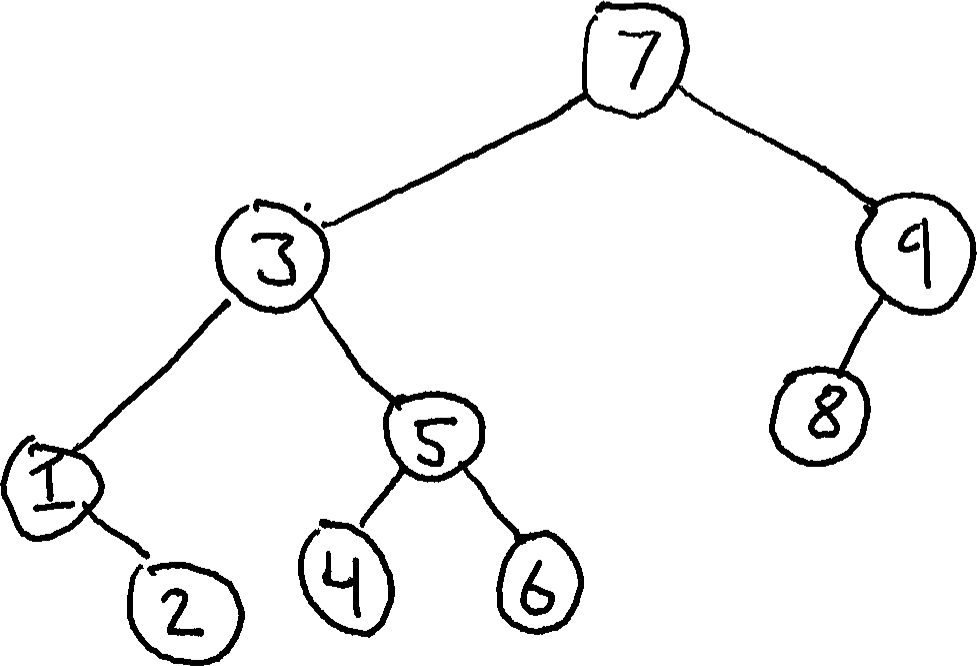
\includegraphics[width=0.6\textwidth]{graphics/L3_trees/quicksort_tree.png}
    \caption[][0cm]{A tree gotten from quicksorting a list of integers in our example.}
    \label{fig:quicksort_tree}
  \end{figure}

  Finally, we need to quicksort the list $9,8$, where we can pick $9$ as our pivot and get $L = 8$, $R = \emptyset$. The resulting tree of what we just did is drawn in Figure \ref{fig:quicksort_tree}.
\end{example}

\section{Exercises}

%\bibliography{references}
%\bibliographystyle{plainnat}

\end{document}
